% -*- coding: utf-8 -*-

\chapter{Resultados}
\label{chap:results}
\drop{E}{n} el siguiente capítulo se describen las iteraciones llevadas a cabo 
para el desarrollo del proyecto. En primer lugar, se exponen los requisitos 
generales del sistema. A continuación, se realizará el análisis de requisitos 
(más específico), el diseño y la implementación de cada una de las iteraciones
programadas. Después, se analizarán las pruebas de campo realizadas sobre
el prototipo final construido. Y por último, se presentará el manual de usuario
de la aplicación, el \emph{diagrama de Gantt} con el seguimiento del proyecto
y la estimación de costes para implantar este sistema en un restaurante real.

\section{Requisitos generales del sistema}
A continuación se listan los requisitos generales que debe satisfacer el
sistema:
\begin{enumerate}
\item Se pretende construir un sistema que siga las líneas maestras que
plantea el modelo de comercio móvil basado en \acs{NFC} (o \acs{NMC}) (ver
capítulo \ref{chap:antecedents}, sección \ref{subsec:related}).
\item El sistema está orientado a implantarse en restaurantes de tipo
\emph{gourmet} o \emph{temático} (ver capítulo \ref{chap:methods}, sección 
\ref{sec:fieldStudy}).
\item El restaurante dispondrá de un terminal en la zona de entrada al salón,
llamada también \emph{recibidor}, que estará regentado por un \emph{maître} y
que se encargará de registrar la entrada y salida de clientes y de procurarles
asiento (ver figura \ref{fig:scenario}, página \pageref{fig:scenario}).
\item El restaurante dispondrá de un terminal en la zona de la \emph{barra}.
Este terminal (a cargo de los camareros) se encargará de gestionar el estado de
los pedidos de los clientes (ver figura \ref{fig:scenario}, página
\pageref{fig:scenario}).
\item El restaurante dispondrá de un servidor de servicios web que podrá o no
estar alojado en uno de los terminales del local. Este servidor se encargará
de dispensar la información que los terminales (\emph{recibidor} y
\emph{barra}) necesitan para trabajar.
\item Los terminales (\emph{recibidor} y \emph{barra}) contarán con una 
conexión directa (mediante \acs{LAN} o conexión directa a internet) con el
servidor de servicios web.
\item Los terminales (\emph{recibidor} y \emph{barra}) contarán con la
tecnología \emph{Bluetooth} que posibilitará las comunicaciones con los
dispositivos móviles.
\item Las mesas del restaurante contarán con un identificador único que
servirá para asociar los pedidos que realiza un cliente con los pedidos que
deben servirse en una mesa.
\item Se ubicará una etiqueta \acs{RFID} cerca del \emph{recibidor}. Esta
etiqueta será usada por los clientes para iniciar la aplicación de su
dispositivo móvil, con objeto de que esta contacte con el terminal del
\emph{recibidor} para registrar su paso por allí. El cliente tocará la
etiqueta al llegar (para registrar su entrada) y al salir (para confirmar
su salida) del establecimiento.
\item Las mesas del restaurante contarán con una carta o menú formado por
etiquetas \acs{RFID}. Cada etiqueta representará a un producto distinto.
Cuando un cliente acerque su dispositivo móvil a una de estas etiquetas,
aparecerá el producto al que representa como un \emph{ítem} de la lista de
productos del pedido.
\item Las cartas o menús dispondrán de otras etiquetas que posibiliten acciones
como: enviar pedido, solicitar factura o decrementar producto. Estas
operaciones permitirán que el usuario se olvide del uso del teclado, ya que
conseguirá todo lo que quiere con sólo acercar su dispositivo a la etiqueta
adecuada.
\item Si el cliente no ha pagado por medios tradicionales e intenta abandonar
el establecimiento, se iniciará el procedimiento de pago mediante \acs{NFC}.
\end{enumerate}

\section{Iteraciones}
Como ya se explicó en la sección \ref{sec:workingMethodology} (página
\pageref{sec:workingMethodology}) el proyecto sigue un desarrollo de
\emph{prototipado incremental}. Por lo tanto, se basa en la consecución de una
serie de fases o iteraciones, a través de las cuales se van incorporando nuevas
funcionalidades hasta obtener el sistema completo.

A continuación, se profundiza en el contenido de cada una de estas fases:

\subsection{Servicios web y base de datos}
Los servicios web se encargarán de atender las solicitudes de información que
demande la \emph{aplicación de la barra} y la \emph{aplicación del recibidor}.
Para asegurar la persistencia de los datos con los que trabaja el restaurante
se hará uso de una base de datos.

\subsubsection{Análisis de requisitos}
Los requisitos específicos de los servicios web y de la base de datos son
los siguientes:
\begin{enumerate}
\item Habrá tres tipos de servicios: los que sólo son accedidos por la
aplicación de la \emph{barra}, los que sólo son accedidos por la aplicación
del \emph{recibidor} y los servicios comunes a ambas.
\item Cada servicio ofrecido estará implementado en un método. Los valores
devueltos por el método sólo pueden ser primitivos (\emph{integer},
\emph{double}, \emph{string}, etc.) por lo que cuando sea necesario devolver
información estructurada se hará uso de cadenas (\emph{string}s) codificadas
en formato \acs{XML}.
\item Entre los servicios que se deben ofrecer están los siguientes:
  \begin{itemize}
  \item Mostrar los tipos de planta de restaurante disponibles.
  \item Devolver la descripción de la planta del restaurante elegido.
  \item Añadir una nueva descripción para la planta del restaurante.
  \item Devolver el estado actual de las mesas.
  \item Ubicar a un nuevo cliente en una mesa vacía.
  \item Desubicar a un cliente existente de su mesa.
  \item Devolver el estado actual de los pedidos.
  \item Registrar nuevo pedido.
  \item Cambiar el estado del pedido.
  \item Calcular la factura para una mesa.
  \item Devolver la lista de productos registrados.
  \item Modificar la lista de productos registrados.
  \end{itemize}
\item El servidor de servicios web asegurará la persistencia de los datos con
los que trabaja a través de una base de datos, que se encontrará en la misma
o en distinta máquina que este.
\item La aplicación de los servicios web será la única que pueda acceder a los
datos de la base de datos.
\item La base de datos almacenará tanto datos estáticos del restaurante (como
nombre, dirección, NIF, teléfono, etc.), como datos dinámicos (estado de los 
pedidos, estado de las mesas, etc.).
\item Los datos estáticos definirán la identidad del restaurante, de los
clientes y de los productos que se ofertan.
\item Los datos dinámicos permitirán llevar un seguimiento del estado actual
del restaurante.
\item En resumen, los datos a almacenar serán los siguientes:
  \begin{itemize}
  \item Datos del restaurante (NIF, nombre, teléfono, mail, IVA, etc.).
  \item Datos de los clientes (DNI, nombre, apellidos, estado, apariciones,
  etc.).
  \item Datos de los productos (nombre, categoría, precio, etc.).
  \item Pedidos registrados durante la sesión.
  \item Descripción de los salones. El salón del restaurante estará
  representado por una serie de objetos que habrán sido definidos por el
  responsable del salón.
  \item Estado de las mesas durante la sesión.
  \item Historial de las facturas pagadas.
  \end{itemize}
\end{enumerate}

\subsubsection{Diseño e implementación}
% Meter diagrama de casos de uso de los servicios web

% Meter diagrama de clases de los servicios web

% Hacer referencia al anexo de los XMLs diseñados para la comunicación con
% las aplicaciones de escritorio.

% Meter diagrama de entidad-interrelación de la base de datos
% Explicar el contenido de cada una de las tablas que forman parte de la BD.

\subsection{\emph{Recibidor} y conexión con servicios web}
La aplicación del \emph{recibidor} se encargará principalmente de registrar a
los clientes que llegan y que salen del restaurante. El prototipo resultante
de esta fase será capaz de registrar la entrada y la salida de clientes que no
hacen uso de la tecnología \acs{NFC}.

\subsubsection{Análisis de requisitos}
Los requisitos específicos de la aplicación del \emph{recibidor} son los
siguientes:
\begin{enumerate}
\item El terminal del recibidor contará con un monitor táctil,
por lo tanto, la aplicación debe estar diseñada teniendo en cuenta que no se
dispone de teclado para la entrada de datos.
\item La aplicación contará con un \emph{editor de escenarios} que permita
definir la distribución de los objetos más característicos que forman
parte del restaurante:
  \begin{itemize}
  \item Se podrán definir las posiciones de cada mesa, del espacio ocupado por
  el recibidor y del espacio ocupado por la barra.
  \item Además cada mesa estará definida también por un identificador único y
  por una capacidad.
  \item Cada tipo de objeto será representado por un color.
  \item El editor permitirá cargar y guardar escenarios. Los escenarios serán
  almacenados en la base de datos a través del servicio web correspondiente.
  \end{itemize}
\item Al iniciar la ejecución, el usuario tendrá dos opciones:
\emph{iniciar una nueva jornada}, que reseteará los datos dinámicos
correspondientes al estado anterior del restaurante (pedidos pendientes y
estado de las mesas); o \emph{iniciar una jornada existente}, que cargará
estos datos.
\item Al \emph{iniciar una nueva jornada}, el usuario elegirá qué planta del
restaurante va a utilizar para representar la distribución actual de los
objetos que hay en él.
\item El estado del restaurante se representará con un mapa similar al mostrado
en el \emph{editor de escenarios}, con la salvedad de que las mesas aparecerán
de un color distinto según su estado.
\item Cada mesa se encontrará en uno de los siguientes estados:
  \begin{itemize}
  \item \textbf{Libre}. Cuando la mesa no está ocupada por ningún cliente.
  \item \textbf{Ocupada}. Cuando la mesa está ocupada por un cliente.
  \item \textbf{Cobrada}. Cuando la mesa está ocupada por un cliente que ya
  ha pagado. Esto implica que el cliente puede abandonar el restaurante
  cuando quiera y que va a dejar la mesa libre.
  \end{itemize}
\item Cada cliente estará representado por un identificador único.
\item Para registrar el ingreso de un nuevo cliente, la aplicación mostrará
las mesas que este puede ocupar, teniendo en cuenta el número de comensales que
son y la capacidad de las mesas.
\item Para confirmar la salida de un cliente, la aplicación sólo dejará
desocupar las mesas que hayan pagado sus pedidos.
%%%%%%% Estadísticas?
%%%%%%% Establece los datos del restaurante?
\end{enumerate}

\subsubsection{Diseño e implementación}
Teniendo en cuenta el análisis de requisitos realizado anteriormente, el
\textbf{diagrama de casos de uso} del prototipo de la aplicación del
\emph{recibidor} quedaría de la siguiente forma (figura \ref{fig:ucdR-phase1}):

  \begin{figure}[!h]
    \begin{center}
      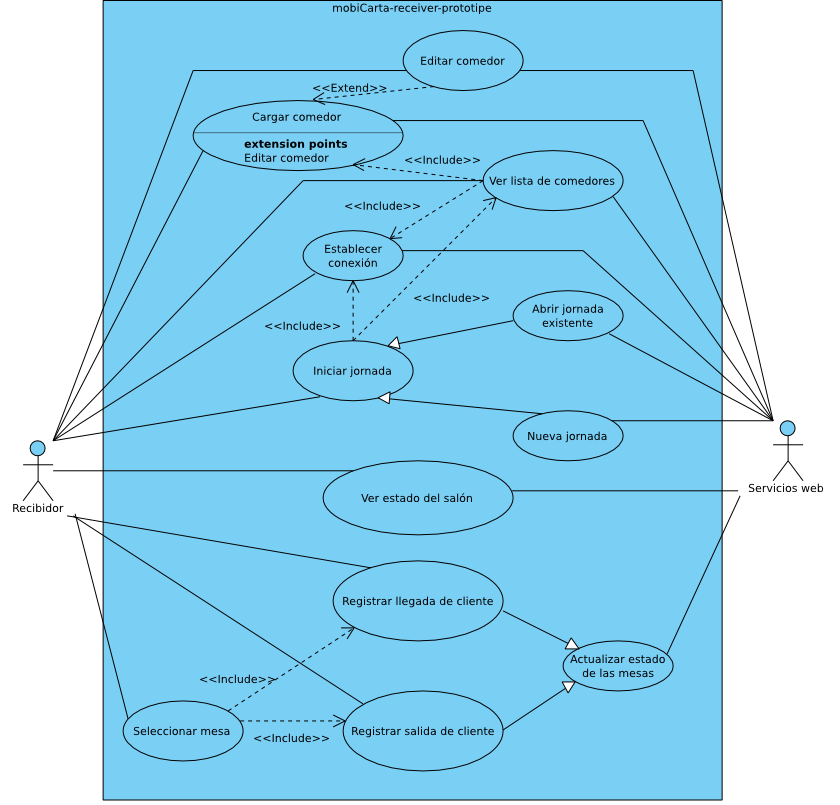
\includegraphics[width=1\textwidth]{ucdR-phase1.png}
      \caption{Diagrama de casos de uso del primer prototipo de la aplicación
      del \emph{recibidor}.}
      \label{fig:ucdR-phase1}
    \end{center}
  \end{figure}

Los principales casos de uso que muestra el diagrama (figura
\ref{fig:ucdR-phase1}) son los siguientes:
\begin{itemize}
\item \textbf{Nueva jornada}. Cuando el \emph{recibidor} quiere iniciar una
nueva jornada (``desde cero''), le pide al \emph{servicio web} que le mande 
una lista con los salones que previamente ha diseñado. De entre todos ellos
elige el que se adapte a la distribución actual de los objetos en el
restaurante y le pide al \emph{servicio web} que le mande la distribución del
salón elegido para cargarlo en pantalla. Una vez cargado, el \emph{recibidor}
vuelve a comunicarse con el \emph{servicio web} para decirle que \emph{resetee}
los valores almacenados de la jornada anterior. La figura \ref{fig:sdR1-phase1}
(página \pageref{fig:sdR1-phase1}) muestra el \textbf{diagrama de secuencia} 
de este caso de uso:

% Todos los diagramas de secuencia deben ir apaisados en páginas aparte.
% Estoy buscando cómo poder hacerlo porque utilizando \begin{sidewaysfigure}
% no me compila bien...

  \begin{figure}[!h]
    \begin{center}
      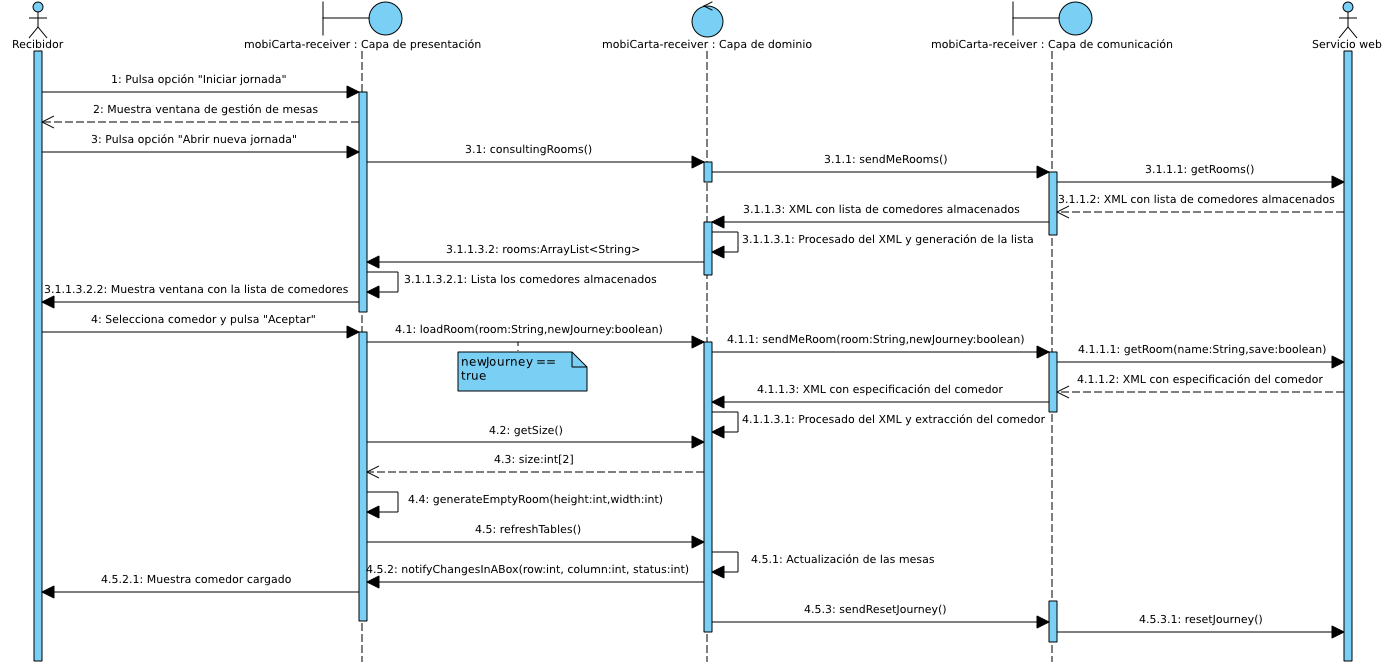
\includegraphics[width=1\textwidth]{sdR1-phase1.png}
      \caption{Diagrama de secuencia del caso de uso \emph{iniciar nueva
      jornada}.}
      \label{fig:sdR1-phase1}
    \end{center}
  \end{figure}

\item \textbf{Abrir jornada existente}. Este caso de uso es similar al
anterior, con la salvedad de que, aquí no se elige el salón a
utilizar (se coge el salón de la jornada anterior). Además, tampoco se
\emph{resetean} los valores almacenados durante dicha jornada. La figura
\ref{fig:sdR2-phase1} (página \pageref{fig:sdR2-phase1}) muestra el
\textbf{diagrama de secuencia} de este caso de uso:

  \begin{figure}[!h]
    \begin{center}
      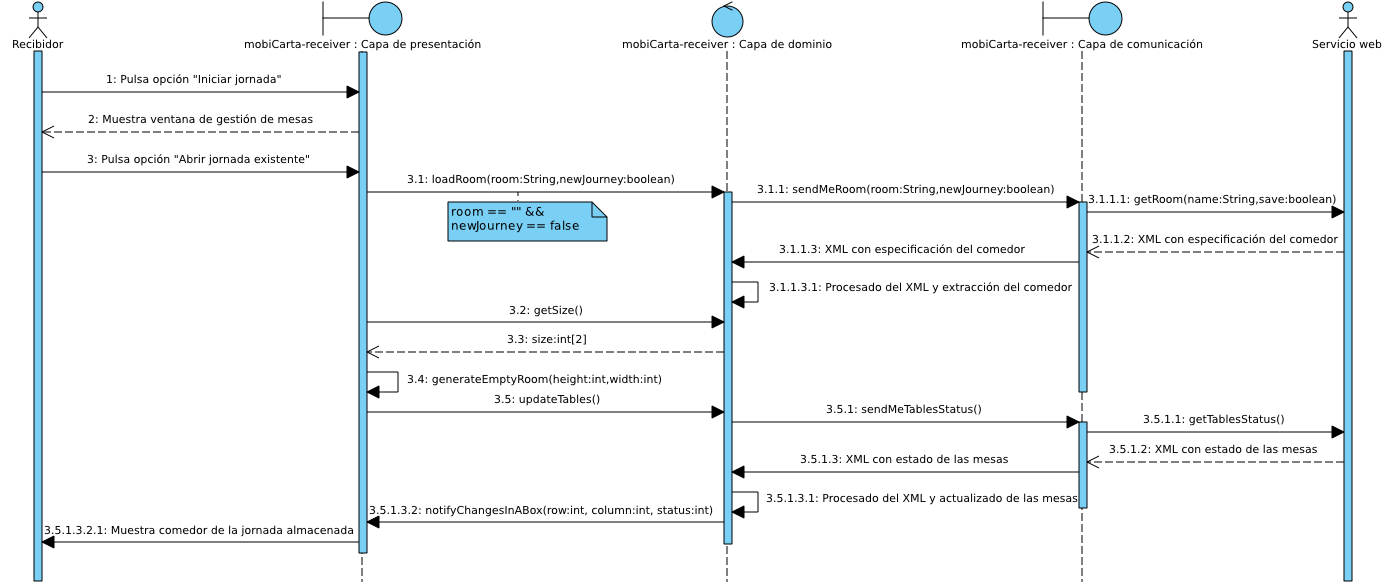
\includegraphics[width=1\textwidth]{sdR2-phase1.png}
      \caption{Diagrama de secuencia del caso de uso \emph{iniciar jornada
      existente}.}
      \label{fig:sdR2-phase1}
    \end{center}
  \end{figure}

\item \textbf{Registrar llegada de cliente}. Este caso de uso hace referencia
a la acción de registrar un nuevo cliente de forma manual
(\emph{no-\acs{NFC}}). Cuando se confirma una nueva llegada, se
genera un identificador único que se le asigna al cliente entrante.
Este identificador tendrá la siguiente forma: un prefijo, 'C'; seguido del
año, mes, día, minuto y segundo en el que se produce el registro. Por ejemplo,
el cliente $C20120720214850$ habrá llegado a las $21:48:50$ del día $20$ de
\emph{Julio} de $2012$. A continuación, el cliente introduce el número de
comensales que son. La aplicación (a través del \emph{servicio web})
comprobará las mesas que están disponibles y que tienen una capacidad
suficiente y las mostrará por pantalla. Por último, se marcará una de las
mesas candidatas y se formalizará con ello el ingreso. Nuevamente el
\emph{servicio web} actualizará el estado de las mesas teniendo en cuenta el
nuevo ingreso. La figura \ref{fig:sdR3-phase1} (página
\pageref{fig:sdR3-phase1}) muestra el \textbf{diagrama de secuencia} de este
caso de uso:

  \begin{figure}[!h]
    \begin{center}
      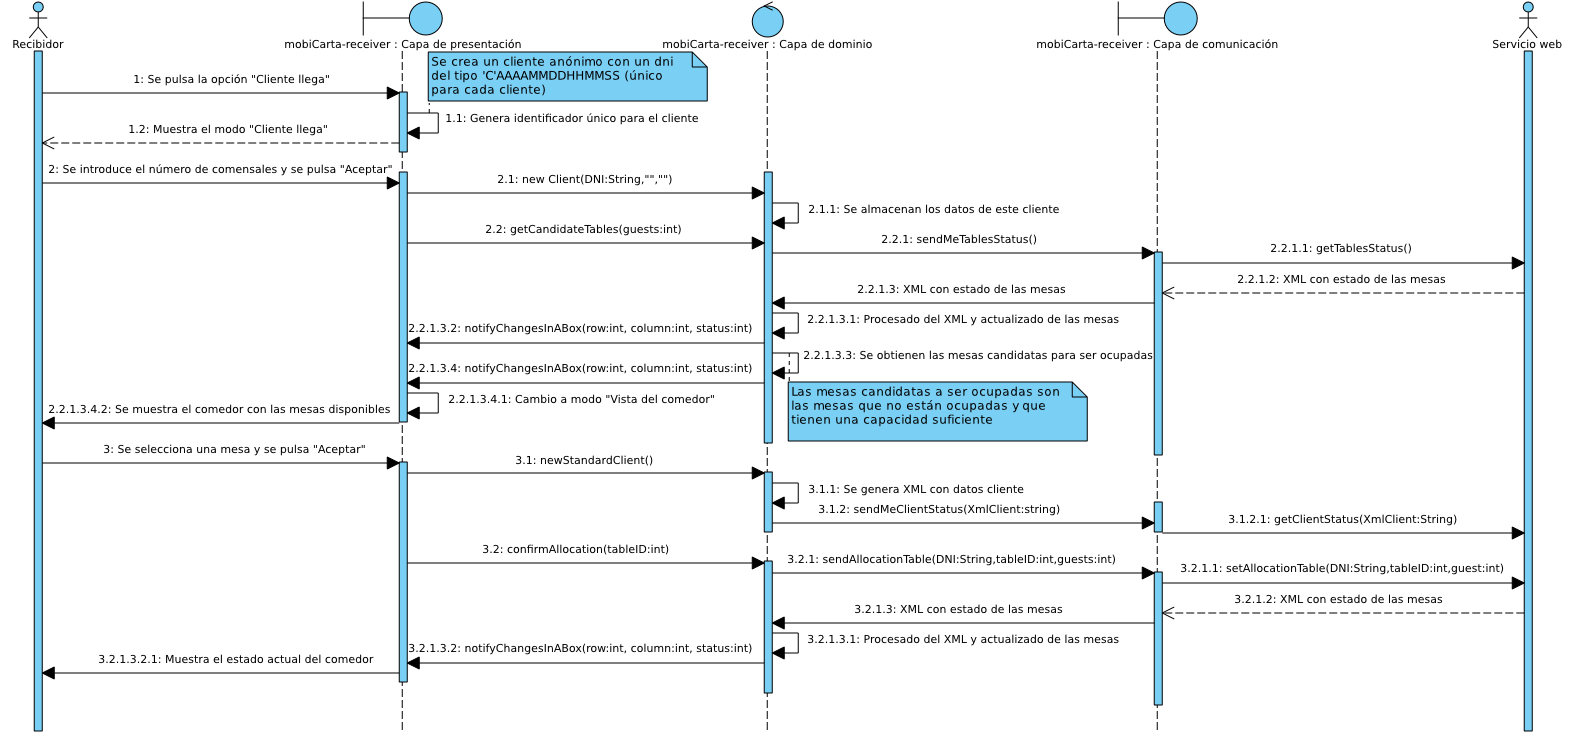
\includegraphics[width=1\textwidth]{sdR3-phase1.png}
      \caption{Diagrama de secuencia del caso de uso \emph{registrar llegada
      de cliente}.}
      \label{fig:sdR3-phase1}
    \end{center}
  \end{figure}

\item \textbf{Registrar salida de cliente}. Para registrar la salida de un
cliente (\emph{normal} o \emph{\acs{NFC}}), simplemente se selecciona la
opción de \emph{Cliente se va}. La aplicación recurre al \emph{servicio web}
para actualizar el estado de las mesas y con ello representa cuáles son las
susceptibles de quedarse vacías. En este caso, las mesas candidatas son
aquellas en las que el cliente ha pagado la cuenta. A continuación, se marca
cuál es la mesa que va a ser abandonada y se pulsa \emph{Aceptar}. Finalmente,
la aplicación avisa al \emph{servicio web} acerca de la mesa que ha quedado
libre y este actualiza el estado del salón. La figura \ref{fig:sdR4-phase1}
(página \pageref{fig:sdR4-phase1}) representa el \textbf{diagrama de secuencia}
del caso de uso \emph{registrar salida de cliente}:

  \begin{figure}[!h]
    \begin{center}
      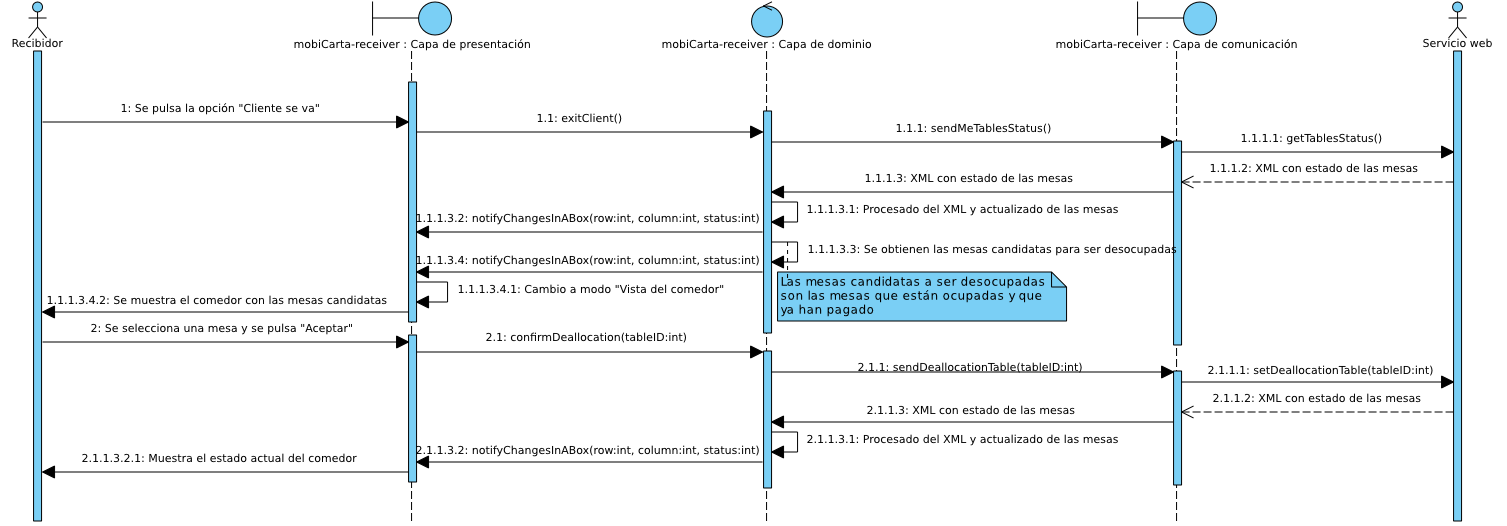
\includegraphics[width=1\textwidth]{sdR4-phase1.png}
      \caption{Diagrama de secuencia del caso de uso \emph{registrar salida
      de cliente}.}
      \label{fig:sdR4-phase1}
    \end{center}
  \end{figure}
\end{itemize}

% Meter diagrama de clases del prototipo

\subsection{\emph{Barra} y conexión con servicios web}
La aplicación de la \emph{barra} se encargará principalmente de gestionar el
estado de los pedidos de los clientes. El prototipo resultante de esta
iteración será capaz de realizar todas las funcionalidades definidas para
los \emph{clientes normales} (ver apartado \emph{Los clientes},
subsección \ref{subsubsec:clients}, página \pageref{subsubsec:clients}).

\subsubsection{Análisis de requisitos}
Los requisitos específicos de la aplicación de la \emph{barra} son los
siguientes:
\begin{enumerate}
\item El terminal de la barra contará con un monitor táctil, por lo que la
aplicación debe estar diseñada teniendo en cuenta que la mayor parte de las
interacciones se realizarán sin hacer uso del teclado.
\item La aplicación contará con un \emph{editor de productos} que permita
definir las características de los productos que hay a la venta:
  \begin{itemize}
  \item Los productos estarán clasificados por categorías, por lo que el
  editor también podrá eliminar, crear y editar nuevas categorías.
  \item El producto quedará identificado por su nombre.
  \item Además del nombre y la categoría, cada producto tendrá otros atributos
  como: el precio, el número de unidades que hay que pedir para obtener un
  descuento (si lo tuviese), el \% de dicho descuento y un atributo
  \emph{booleano} que determine si el producto aparecerá como visible o no
  visible a la hora de realizar pedidos.
  \end{itemize}
\item Como ocurría con la aplicación del \emph{recibidor}, la aplicación de la
\emph{barra} también tiene dos opciones: \emph{iniciar una nueva jornada} e
\emph{iniciar una jornada existente}. El funcionamiento es el mismo que las
funciones homónimas ya comentadas.
\item El estado del restaurante se muestra de forma similar a como lo hace
la aplicación del \emph{recibidor}, con la salvedad de que ahora las mesas
tienen otros estados:
  \begin{itemize}
  \item \textbf{Libre}. La mesa no está ocupada por ningún cliente.
  \item \textbf{Ocupada}. La mesa está ocupada por un cliente que no ha
  realizado aún ningún pedido.
  \item \textbf{Esperando}. El cliente de dicha mesa ha realizado un pedido y
  este aún no ha sido entregado.
  \item \textbf{Atendida}. Todos los pedidos que ha hecho el cliente de esta
  mesa han sido atendidos.
  \item \textbf{Cobrada}. Los pedidos de esta mesa han sido cobrados, pero el
  cliente aún no la ha abandonado.
  \end{itemize}
\item La aplicación debe tener la funcionalidad para anotar pedidos similar a 
las ya vistas en otros gestores de restaurantes (ver figuras
\ref{fig:productsPanel}, \ref{fig:productsPanel2} y \ref{fig:productsList},
página \pageref{fig:productsPanel}).
\item La aplicación mostrará una lista con todos los pedidos que han sido
realizados durante la sesión.
\item Los pedidos podrán encontrarse en uno de estos estados:
  \begin{itemize}
  \item \textbf{No atendido}. Se ha tomado nota del pedido pero nadie se está
  haciendo cargo de él.
  \item \textbf{Atendido}. En caso de que el producto tenga que ser elaborado
  (por un cocinero, por ejemplo), este estado determina que el plato está
  siendo cocinado.
  \item \textbf{Servido}. Cuando el producto ha llegado a su destinatario, el
  estado del producto debe cambiarse a \emph{servido}.
  \item \textbf{Detenido}. En caso de producirse alguna incidencia con el
  pedido (por ejemplo, falta alguna materia prima para elaborar
  el plato pero se repondrá en breve), es conveniente contar con un estado
  de \emph{excepción}.
  \item \textbf{Cobrado}. Para identificar que los pedidos de esa mesa ya han
  sido cobrados.
  \end{itemize}
\item La aplicación podrá mostrar la situación de una mesa en concreto: quién
la ocupa, en qué estado se encuentra, cuáles son sus pedidos, cuál es el
estado de dichos pedidos, etc.
\item Cuando todos los pedidos de una mesa han sido atendidos, se dará la
opción de \emph{facturar} la mesa. Los datos personales suministrados por el
cliente y los datos fiscales de la empresa almacenados en la base de datos
servirán para generar la factura.
%%%%%%% Meter Estadísticas de uso, si da tiempo
\end{enumerate}

\subsubsection{Diseño e implementación}
Teniendo en cuenta el análisis de requisitos realizado anteriormente, el
\textbf{diagrama de casos de uso} del prototipo de la aplicación de la
\emph{barra} queda de la siguiente forma (figura \ref{fig:ucdB-phase2}):

  \begin{figure}[!h]
    \begin{center}
      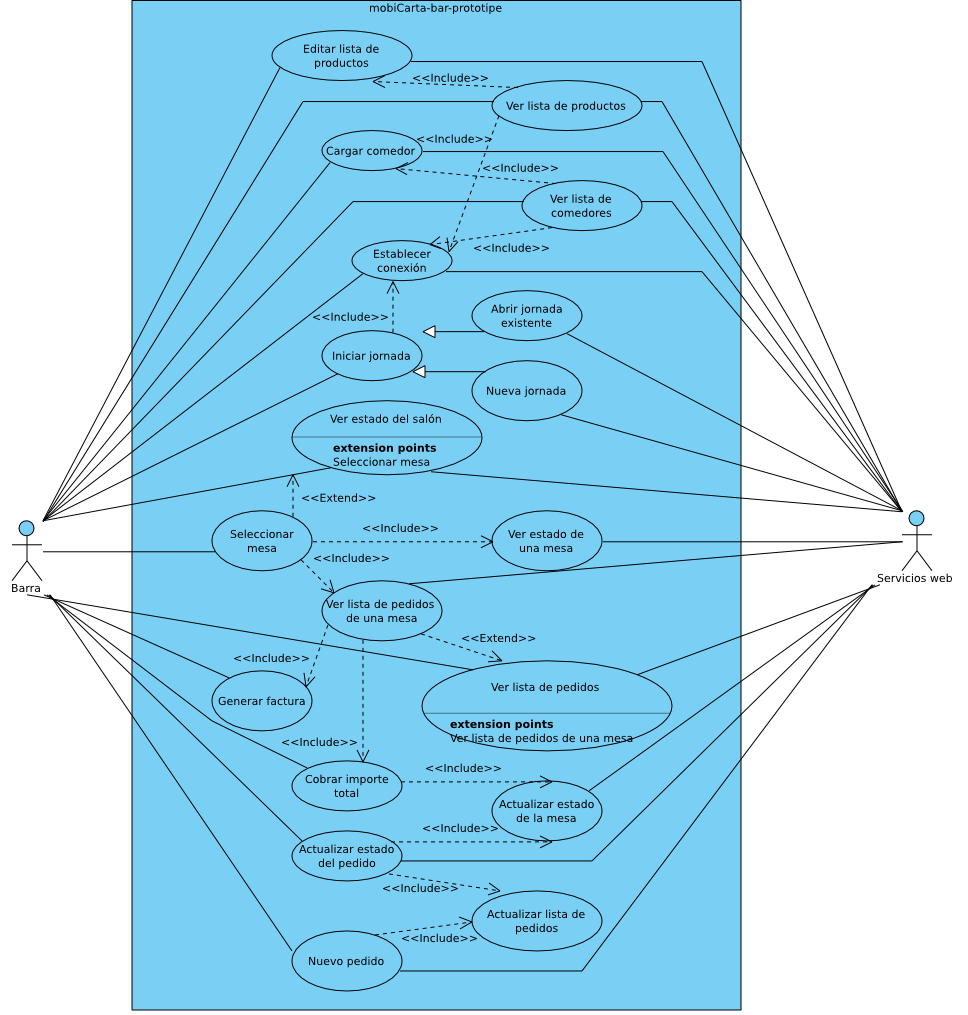
\includegraphics[width=1.1\textwidth]{ucdB-phase2.png}
      \caption{Diagrama de casos de uso del primer prototipo de la aplicación
      de la \emph{barra}.}
      \label{fig:ucdB-phase2}
    \end{center}
  \end{figure}

Los casos de uso más característicos de la aplicación de la \emph{barra} son
los siguientes:
\begin{itemize}
\item Los casos de uso \textbf{Nueva jornada} y \textbf{Abrir jornada
existente} son exactamente iguales que los ya explicados en la aplicación
del \emph{recibidor}. Por lo tanto, los diagramas de secuencia van a ser 
idénticos a los de las figuras \ref{fig:sdR1-phase1} (página
\pageref{fig:sdR1-phase1}) y \ref{fig:sdR2-phase1} (página
\pageref{fig:sdR2-phase1}), respectivamente.
\item \textbf{Ver estado de una mesa}. Durante una jornada activa se tiene
la posibilidad de observar el estado actual del salón. Para ello simplemente
hay que seleccionar la opcion \emph{Mostrar salón}. Para conocer el estado
actualizado del salón, la aplicación echa mano del \emph{servicio web}.
La vista del salón da la posibilidad de seleccionar las mesas ocupadas. Como
ocurre con el estado del salón, la aplicación recurre nuevamente al
\emph{servicio web} para conocer el estado actualizado de la mesa seleccionada.
Esta información incluye: estado de la mesa, cliente que la ocupa, número
de comensales y los pedidos (y su estado) que ha realizado. La figura
\ref{fig:sdB1-phase2} (página \pageref{fig:sdB1-phase2}), muestra el
\textbf{diagrama de secuencia} de este caso de uso:

  \begin{figure}[!h]
    \begin{center}
      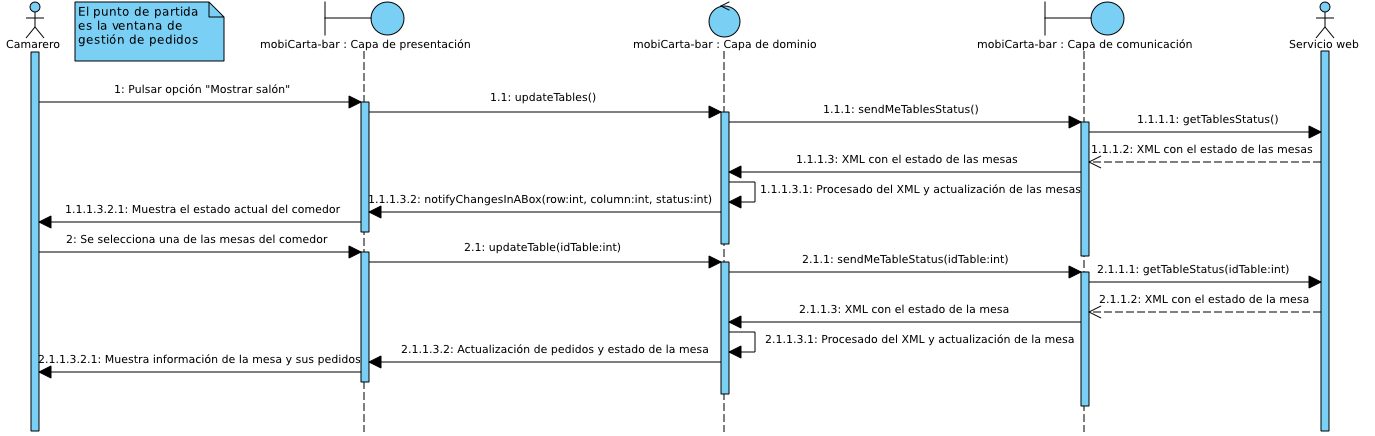
\includegraphics[width=1\textwidth]{sdB1-phase2.png}
      \caption{Diagrama de secuencia del caso de uso \emph{Ver estado de
      una mesa}.}
      \label{fig:sdB1-phase2}
    \end{center}
  \end{figure}

\item \textbf{Nuevo pedido}. Al seleccionar el botón de \emph{añadir pedido}
la aplicación carga una lista con las mesas activas y otra lista con los
productos disponibles. Para asignar un pedido a una mesa: en primer lugar, se
selecciona la mesa de destino; a continuación, se selecciona la categoría
del producto que se pretende añadir; después, se elige la cantidad de
productos que van a añadirse; y por último, se selecciona el producto y se
pulsa \emph{añadir}. La lista de productos generada se le asignará a la mesa
al pulsar \emph{Aceptar}. Este nuevo pedido se envía (en formato \acs{XML})
al \emph{servicio web}. La figura \ref{fig:sdB2-phase2} (página
\pageref{fig:sdB2-phase2}) muestra el \textbf{diagrama de secuencia} de dicho
caso de uso:

  \begin{figure}[!h]
    \begin{center}
      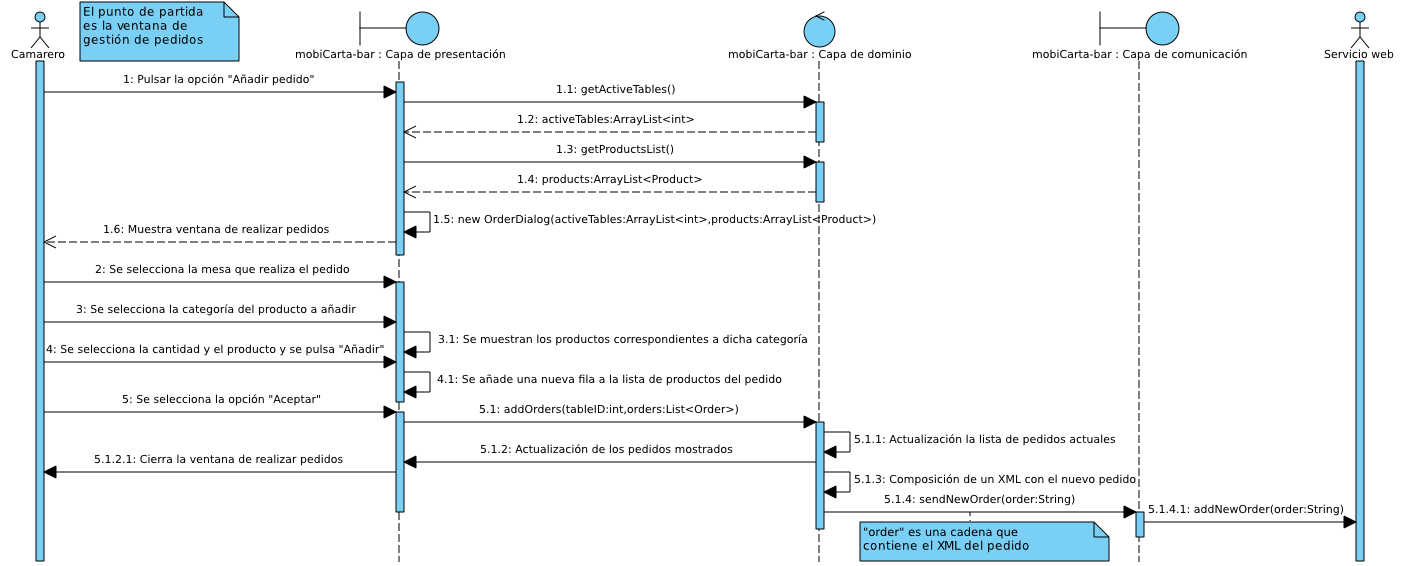
\includegraphics[width=1\textwidth]{sdB2-phase2.png}
      \caption{Diagrama de secuencia del caso de uso \emph{añadir un nuevo
      pedido (manual)}.}
      \label{fig:sdB2-phase2}
    \end{center}
  \end{figure}

\item \textbf{Actualizar el estado de un pedido}. Para cambiar el estado de
un pedido, hay que seleccionarlo en la lista de pedidos y pulsar después uno
de los estados disponibles (\emph{No atendido}, \emph{Atendido},
\emph{Servido}, o \emph{Detenido}). El pedido cambiará de color y se informará
al \emph{servicio web} que dicho cambio.
La figura \ref{fig:sdB3-phase2} (página \pageref{fig:sdB3-phase2}) muestra
un \textbf{diagrama de secuencia} en el que, primero, se cambia el estado de
un producto de \emph{No atendido} a \emph{Atendido}, para informar de que
el pedido está siendo elaborado; y posteriormente se cambia de \emph{Atendido}
a \emph{Servido}, para indicar que el pedido ha sido entregado a la mesa.

  \begin{figure}[!h]
    \begin{center}
      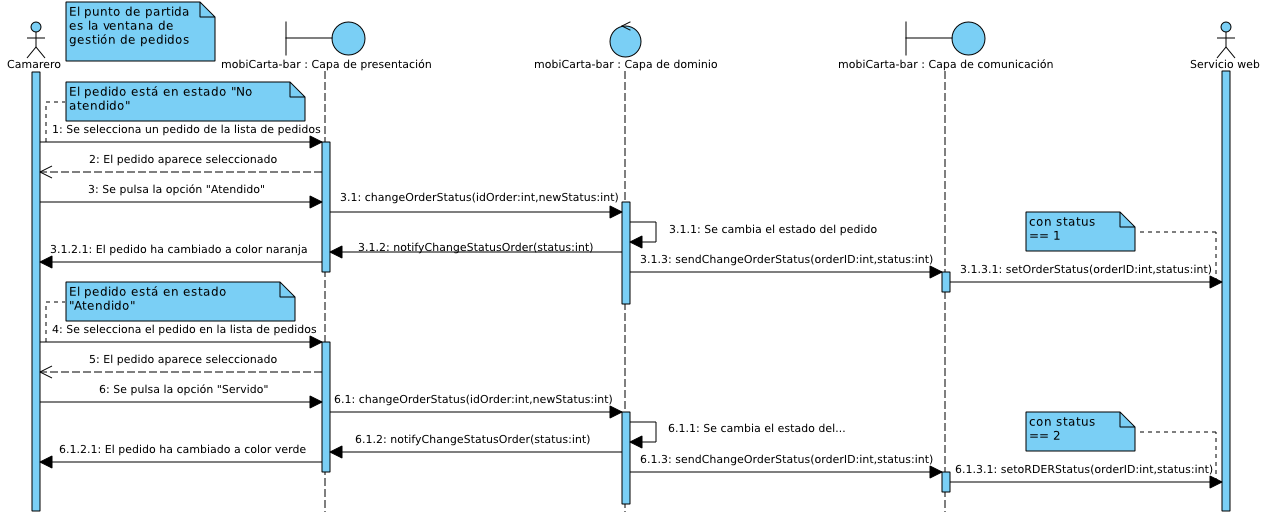
\includegraphics[width=1\textwidth]{sdB3-phase2.png}
      \caption{Diagrama de secuencia del caso de uso \emph{actualizar
      estado de un pedido} de \emph{No atendido} a \emph{Servido}.}
      \label{fig:sdB3-phase2}
    \end{center}
  \end{figure}

\item \textbf{Generar factura} y  \textbf{Cobrar importe total}. Para
facturar una mesa, primero hay que asegurarse de que todos sus pedidos han
sido servidos. Después hay que situarse en la \emph{vista de esa mesa}.
Al pulsar la opción \emph{Facturar}, la aplicación buscará, entre las facturas
generadas, si ha generado la de esa mesa. En caso de no encontrarla recurrirá
al \emph{servicio web}, que es el que en verdad genera las facturas. El
\emph{servicio web} devolverá un \acs{XML} con la factura para esa mesa y la 
aplicación se encargará de decodificarla para crear un objeto de tipo
\emph{Bill}, lo almacenará con el resto de facturas generadas y compondrá
una ventana emergente con los datos de la factura. Una de las opciones de
esa ventana emergente será la de \emph{Pagado}. Con ella se confirmará que
el importe que debe la mesa se ha abonado. La aplicación marcará los
pedidos para esa mesa como \emph{Pagado}s y se informará al \emph{servicio
web} de esta operación. El \emph{servicio web} marcará también esos pedidos
como \emph{Pagado}s, los sacará de la tabla \emph{Orders} y los meterá en
\emph{Historical} y devolverá un \acs{XML} con el nuevo estado del
restaurante. La figura \ref{fig:sdB4-phase2} (página \pageref{fig:sdB4-phase2})
muestra el \textbf{diagrama de secuencia} de estos dos casos de uso:

  \begin{figure}[!h]
    \begin{center}
      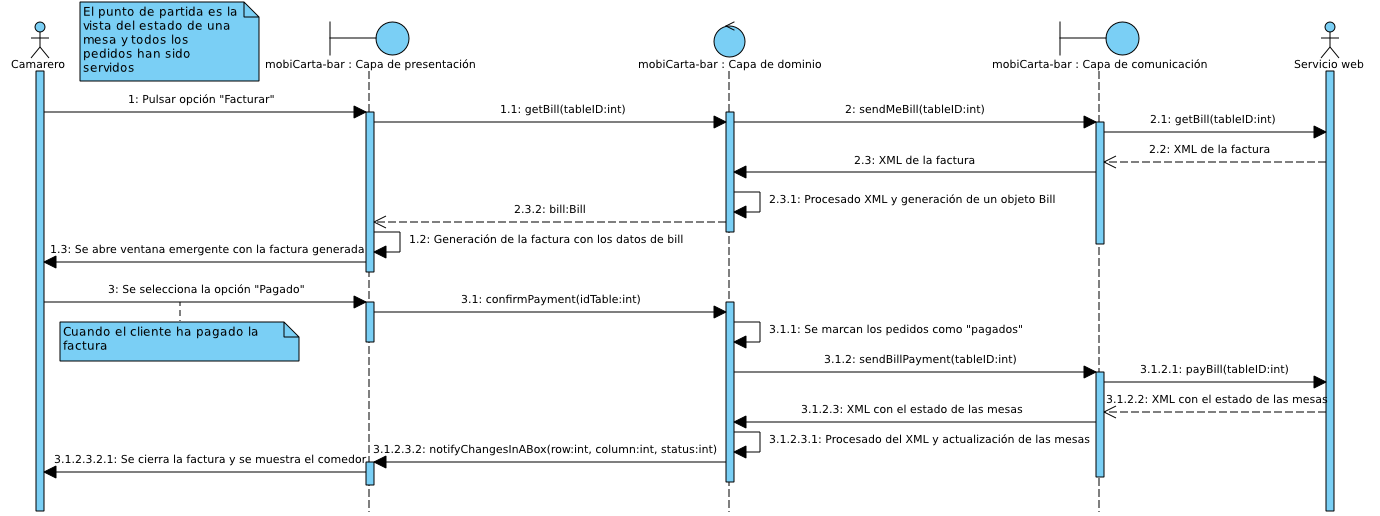
\includegraphics[width=1\textwidth]{sdB4-phase2.png}
      \caption{Diagrama de secuencia del caso de uso \emph{generar factura}
      y \emph{cobrar importe total}.}
      \label{fig:sdB4-phase2}
    \end{center}
  \end{figure}
\end{itemize}

% Meter diagrama de clases del prototipo

\subsection{Aplicación móvil}
Esta es la aplicación destinada a los clientes y les servirá para interactuar
directamente con el restaurante. En esta fase se pretende construir un
prototipo que sea capaz de interactuar con los distintos
tipos de etiquetas \acs{RFID} que se definan.

\subsubsection{Análisis de requisitos}
Los requisitos específicos que se definen para la aplicación móvil son los
siguientes:
\begin{enumerate}
\item La aplicación móvil tiene por objetivo comunicar al cliente con el
restaurante utilizando básicamente dos tecnologías inalámbricas: \acs{NFC} y
\emph{Bluetooth}. Por lo tanto, es condición indispensable que el dispositivo
móvil disponga de esas tecnologías.
\item Antes de realizar cualquier interacción con el restaurante, el cliente
debe rellenar un formulario con sus datos personales. Estos datos servirán para 
poder identificar al usuario. Los datos serán guardados en algún lugar del
dispositivo para poder recuperarlos cuando hagan falta.
\item Debido al pequeño tamaño de la pantalla de los dispositivos móviles, las 
pantallas que forman la \acs{GUI} de la aplicación deben tener un diseño 
minimalista. Es decir, deben representar sólo la información necesaria en cada
momento, evitando sobrecargar la pantalla con elementos innecesarios.
\item Todas las interaciones simples deben poder realizarse utilizando
únicamente la tecnología \acs{NFC}. Se pretende así evitar el hacer uso del
teclado. Las interacciones son las siguientes:
  \begin{itemize}
  \item Registrar el paso del cliente por la zona del \emph{recibidor}.
  Según el estado del cliente (almacenado por el sistema), significará: que
  el cliente ha llegado al restaurante, que el cliente abandona el restaurante
  o bien que el cliente desea pagar mediante \acs{NFC}.
  \item Leer el contenido de las etiquetas del menú para elaborar una lista
  de productos para un pedido.
  \item Dar la posibilidad de decrementar el número de productos de un tipo
  sin utilizar el teclado.
  \item Enviar el pedido a la aplicación de la \emph{barra}.
  \item Solicitar la cuenta total de los pedidos realizados.
  \end{itemize}
\item Existirá un tipo de etiqueta por cada interacción simple diferente
(es decir, cinco).
\item El contacto con algunas de estas etiquetas provocará el arranque
automático de la aplicación móvil. En concreto estas etiquetas son: la que
registra el paso del cliente por la zona del \emph{recibidor}, cada una de las
etiquetas que representan a los productos del menú y la que permite solicitar
la cuenta.
\end{enumerate}

\subsubsection{Diseño e implementación}
Teniendo en cuenta el análisis de requisitos realizado anteriormente, el
\textbf{diagrama de casos de uso} del prototipo de la aplicación móvil queda
de la siguiente forma (figura \ref{fig:ucdM-phase3}):

  \begin{figure}[!h]
    \begin{center}
      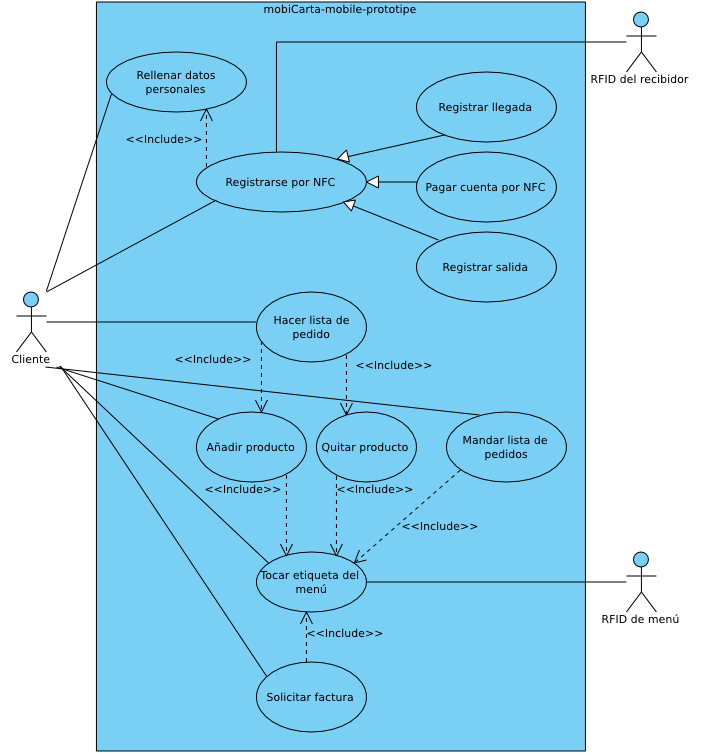
\includegraphics[width=1\textwidth]{ucdM-phase3.png}
      \caption{Diagrama de casos de uso del primer prototipo de la aplicación
      móvil.}
      \label{fig:ucdM-phase3}
    \end{center}
  \end{figure}

Los principales casos de uso serán explicados en las secciones
\ref{subsec:mobile-receiver} y \ref{subsec:mobile-bar} cuando se
definan las comunicaciones \emph{Bluetooth} entre la aplicación móvil y
la aplicación del recibidor y de la barra.

El anexo \ref{chap:tags} muestra los distintos tipos de etiquetas definidos y
su distribución dentro del restaurante.

% Meter diagrama de clases del prototipo

\subsection{Comunicación \emph{Bluetooth} entre móvil y \emph{recibidor}}
\label{subsec:mobile-receiver}
La comunicación \emph{Bluetooth} entre el dispositivo móvil y la aplicación
del \emph{recibidor} posibilitará la autentificación del cliente \acs{NFC}
ante el sistema.

\subsubsection{Análisis de requisitos}
Los requisitos que deben cumplir las comunicaciones \emph{Bluetooth} entre
los dispositivos móviles y la aplicación del \emph{recibidor} son los
siguientes:
\begin{enumerate}
\item La aplicación del dispositivo móvil será la que inicie siempre la
comunicación \emph{Bluetooth}.
\item La comunicación se iniciará cuando el cliente toque con su dispositivo
móvil la etiqueta \emph{RFID} que se encuentra en la zona del \emph{recibidor}.
\item La comunicación consistirá en un mensaje enviado por parte de la
aplicación móvil y la respuesta a este mensaje por parte de la aplicación
del \emph{recibidor}.
\item La aplicación móvil siempre enviará los mismos datos, o lo que es lo
mismo, siempre enviará los datos personales del cliente. Estos datos los
mandará como una cadena codificada con formato \acs{XML}.
\item La respuesta de la aplicación del \emph{recibidor} dependerá del estado
del cliente (\emph{el cliente llega}, \emph{el cliente paga} o \emph{el cliente
se va}). En principio, la respuesta va a consistir en una cadena con un texto
que indique que la operación se ha realizado de forma satisfactoria.
\item A la hora de establecer una conexión, la aplicación móvil no buscará una
dirección \emph{Bluetooth} física concreta, sino que buscará un servicio que
tenga un identificador concreto conocido por esta.
\end{enumerate}

\subsubsection{Diseño e implementación}
Al \textbf{diagrama de casos de uso} de la aplicación del \emph{recibidor}
visto en la primera fase (figura \ref{fig:ucdR-phase1}) se le añaden los
siguientes casos de uso (figura \ref{fig:ucdR-phase4}).

  \begin{figure}[!h]
    \begin{center}
      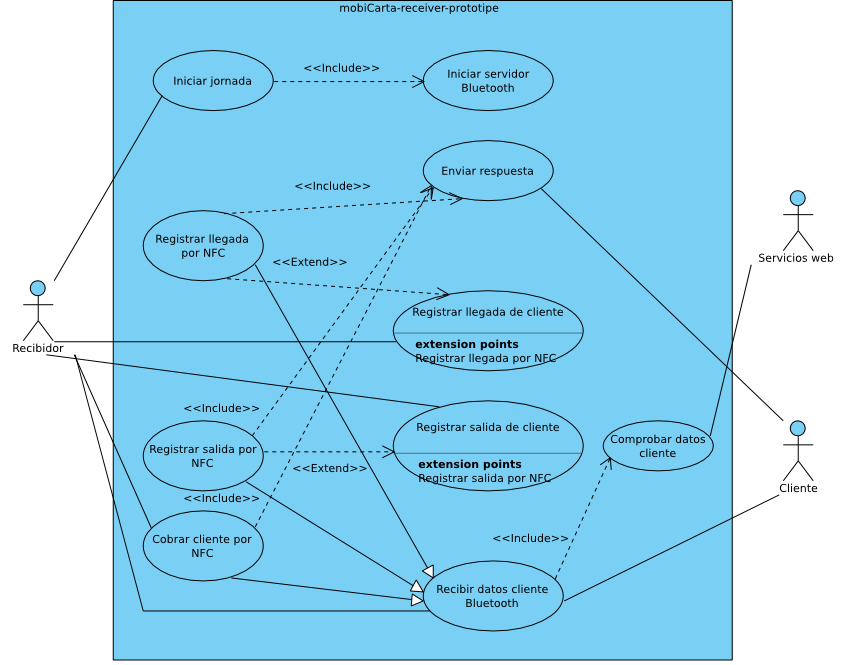
\includegraphics[width=1\textwidth]{ucdR-phase4.png}
      \caption{Casos de uso añadidos al prototipo de la aplicación
      del \emph{recibidor} en esta iteración.}
      \label{fig:ucdR-phase4}
    \end{center}
  \end{figure}

Cuando se lleva a cabo \emph{iniciar jornada}, la aplicación inicia un
\emph{servidor Bluetooth} que se encarga de ofrecer un servicio a los
\emph{clientes \acs{NFC}}. Este servicio está preparado para recibir
los datos personales de los \emph{clientes \acs{NFC}} que pasan por la
zona del \emph{recibidor}, ya sea para registrar su entrada, su intención de
pagar vía \acs{NFC} o su salida. La figura \ref{fig:sdR-phase4} (página
\pageref{fig:sdR-phase4}) muestra el \textbf{diagrama de secuencia} del
caso de uso \emph{registrar salida por \acs{NFC}}.

  \begin{figure}[!h]
    \begin{center}
      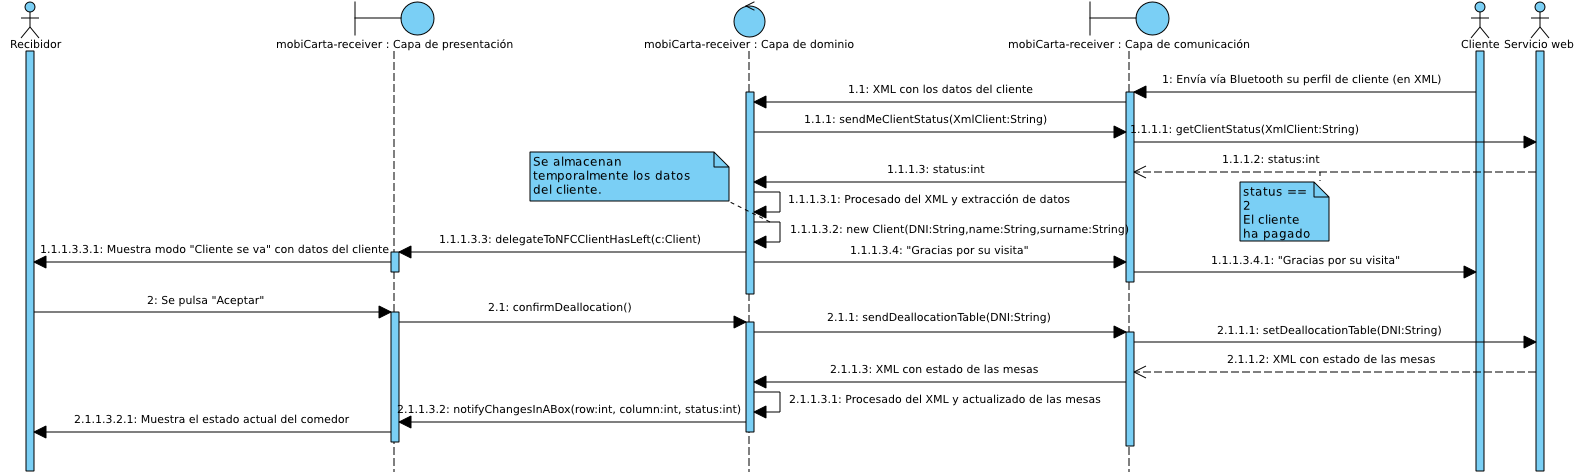
\includegraphics[width=1\textwidth]{sdR-phase4.png}
      \caption{Diagrama de secuencia del caso de uso \emph{registrar salida
      por \acs{NFC}}.}
      \label{fig:sdR-phase4}
    \end{center}
  \end{figure}

Cuando el servidor \emph{Bluetooth} recibe los datos de un usuario (en formato
\acs{XML}), los envía al \emph{servicio web}, para que este le informe del
estado del cliente (\emph{cliente que llega}, \emph{cliente que paga} o
\emph{cliente que se va}). En este caso el cliente se va, por lo tanto la
aplicación del \emph{recibidor} muestra una mensaje emergente informando
del cliente que se va. Por otro lado, el servidor \emph{Bluetooth} le manda
al cliente la confirmación un mensaje tipo \emph{gracias por su visita}.
El \emph{maître}, encargado de manejar la aplicación del \emph{recibidor},
debe confirmar finalmente que el cliente se ha ido. Al hacerlo, informa
al \emph{servicio web} que el cliente ha abandonado su mesa y este le
devuelve la nueva situación del restaurante.

Por otro lado, al \textbf{diagrama de casos de uso} de la aplicación móvil
hay que añadirle los siguientes casos de uso (figura \ref{fig:ucdM-phase4}):

  \begin{figure}[!h]
    \begin{center}
      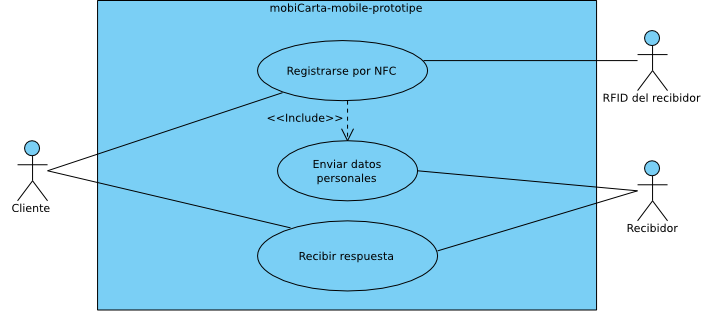
\includegraphics[width=0.9\textwidth]{ucdM-phase4.png}
      \caption{Casos de uso añadidos al prototipo de la aplicación
      móvil en esta iteración.}
      \label{fig:ucdM-phase4}
    \end{center}
  \end{figure}

Los casos de uso \textbf{registrar llegada}, \textbf{pagar cuenta por
\acs{NFC}} y \textbf{registrar salida}, que forman parte de la generalización
de \textbf{Registrarse por \acs{NFC}}, son llevados a cabo por parte del
cliente de forma casi idéntica, ya que el que determina el caso de uso que
se está realizando es la aplicación del \emph{recibidor}. La figura
\ref{fig:sdM-phase4} (página \pageref{fig:sdM-phase4}) muestra el
\textbf{diagrama de secuencia} del caso de uso \emph{registrar entrada}:

  \begin{figure}[!h]
    \begin{center}
      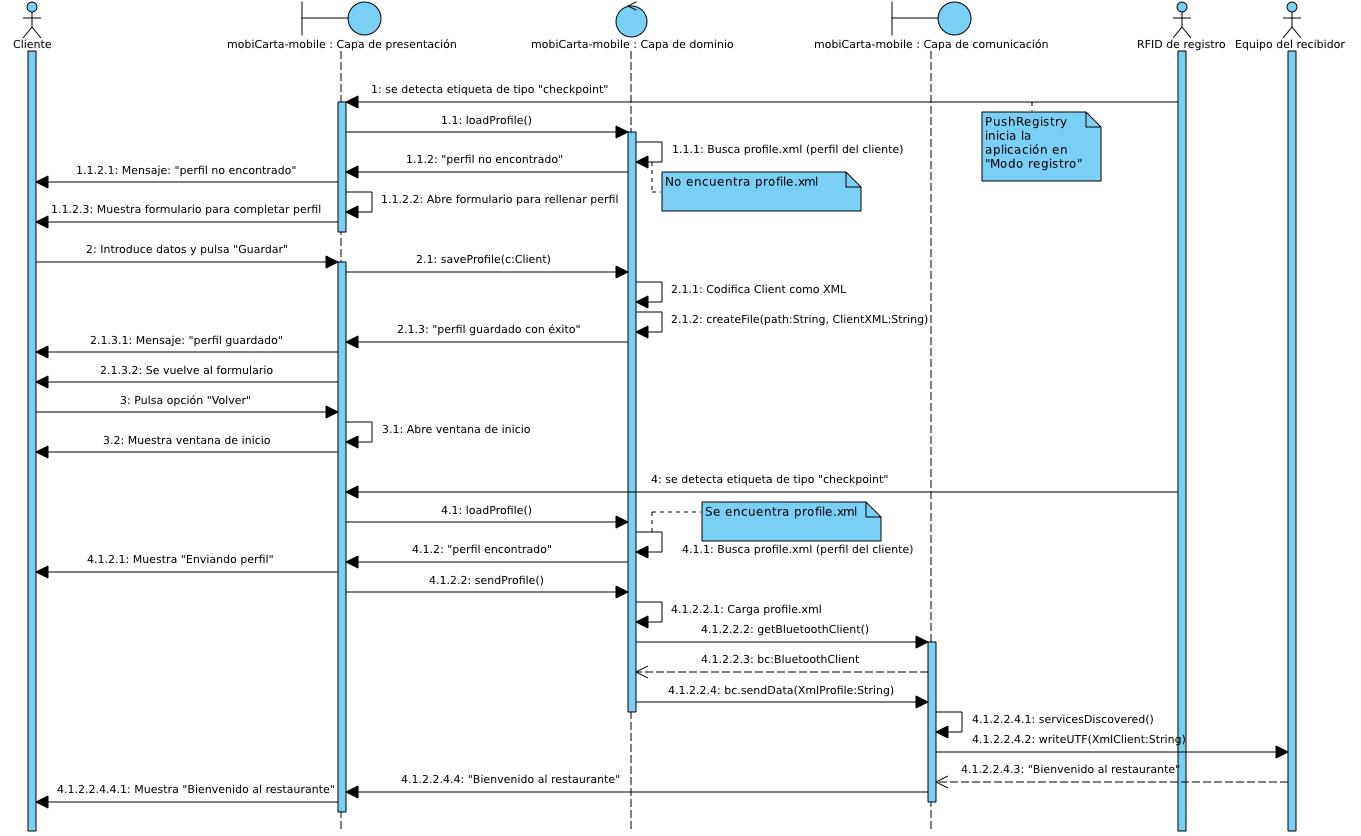
\includegraphics[width=1\textwidth]{sdM-phase4.png}
      \caption{Diagrama de secuencia del caso de uso \emph{registrar entrada},
      de la aplicación móvil.}
      \label{fig:sdM-phase4}
    \end{center}
  \end{figure}

Cuando el móvil se acerca a una etiqueta de tipo \emph{checkpoint}, se
arranca automáticamente la aplicación móvil en \emph{modo registro}. Lo
primero que se comprueba es que existe un archivo llamado \emph{profile.xml},
que guarda la información de usuario del cliente. En caso de no encontrarlo,
la aplicación insta al cliente a que rellene un formulario con sus datos.
Una vez completados, el usuario pulsa la opción \emph{Guardar} y la
aplicación se encarga de codificar la información en formato \acs{XML} y de
guardarla en \emph{profile.xml}. Para volver a intentar registrarse en el
sistema, el cliente deberá aproximar de nuevo su móvil a la etiqueta
\emph{checkpoint}. Esta vez, la aplicación encontrará el archivo
\emph{profile.xml}, cargará su información y buscará el servicio
\emph{Bluetooth} que ofrece la aplicación del \emph{recibidor} para
registrar clientes. Cuando lo encuentre, le mandará la cadena con los datos
del cliente. Finalmente, la aplicación del \emph{recibidor} confirmará que
le ha llegado la información del cliente y que por tanto ha quedado
registrada, en este caso, la entrada al restaurante.

% Meter modificaciones del diagrama de clases del prototipo del recibidor
% y del prototipo móvil.

\subsection{Comunicación \emph{Bluetooth} entre móvil y \emph{barra}}
\label{subsec:mobile-bar}
La comunicación \emph{Bluetooth} entre el dispositivo móvil y la aplicación
de la \emph{barra} permitirá al cliente \acs{NFC} realizar pedidos y conocer
cuál es el importe de la cuenta, sin necesidad de avisar a ningún camarero.

\subsubsection{Análisis de requisitos}
Los requisitos que deben cumplir las comunicaciones \emph{Bluetooth} entre
los dispositivos móviles y la aplicación de la \emph{barra} son los
siguientes:
\begin{enumerate}
\item La aplicación del dispositivo móvil será la que inicie siempre la
comunicación \emph{Bluetooth}.
\item La comunicación se iniciará cuando el cliente confirme (a través de la
etiqueta correspondiente) que va a realizar un pedido con los productos que ha 
ido seleccionando de la carta de etiquetas \acs{RFID}. También puede iniciar
una comunicación para solicitar la cuenta de lo que ha consumido.
\item Todas las comunicaciones consistirán en un mensaje enviado por parte de
la aplicación móvil y la respuesta a este por parte de la aplicación de la
\emph{barra}.
\item La aplicación móvil enviará un mensaje con el identificador del cliente
y los productos (y la cantidad de cada uno de ellos) que forman parte del
pedido o, en caso de solicitar la cuenta, simplemente el identificador del
cliente y el concepto \emph{facturar mesa}. Estos datos los mandará como una
cadena codificada con formato \acs{XML}.
\item La respuesta de la aplicación de la \emph{barra} consistirá en una cadena 
con un texto que indique si la operación se ha completado o no 
satisfactoriamente.
Para la respuesta ante una solicitud de facturación, la aplicación calculará
el importe total de lo que debe la mesa y enviará un resumen (codificado
en formato \acs{XML}) con los productos consumidos y la cantidad a abonar.
\item A la hora de establecer una conexión, la aplicación móvil no buscará una
dirección \emph{Bluetooth} física concreta, sino que buscará un servicio que
tenga un identificador concreto conocido por esta (distinto al servicio
ofrecido por la aplicación del \emph{recibidor}).
\end{enumerate}

\subsubsection{Diseño e implementación}
El \textbf{diagrama de casos de uso} del prototipo de la aplicación de la
\emph{barra} va a ser complementado con los siguientes casos de uso (figura
\ref{fig:ucdB-phase5}):

  \begin{figure}[!h]
    \begin{center}
      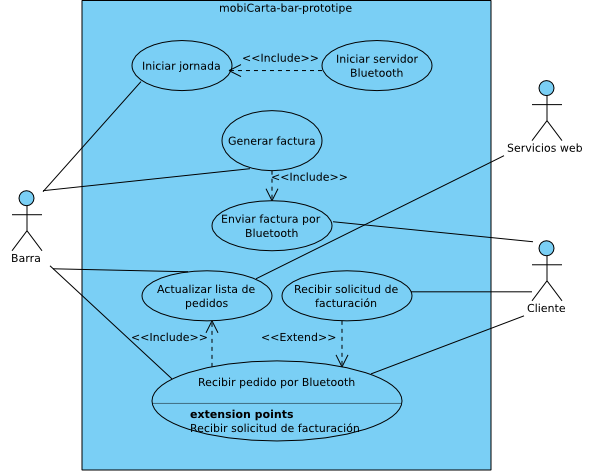
\includegraphics[width=0.8\textwidth]{ucdB-phase5.png}
      \caption{Casos de uso añadidos al prototipo de la aplicación
      de la \emph{barra} en esta iteración.}
      \label{fig:ucdB-phase5}
    \end{center}
  \end{figure}

Por su parte, el \textbf{diagrama de casos de uso} de la aplicación móvil
añade los siguientes casos de uso (figura \ref{fig:ucdM-phase5}):

  \begin{figure}[!h]
    \begin{center}
      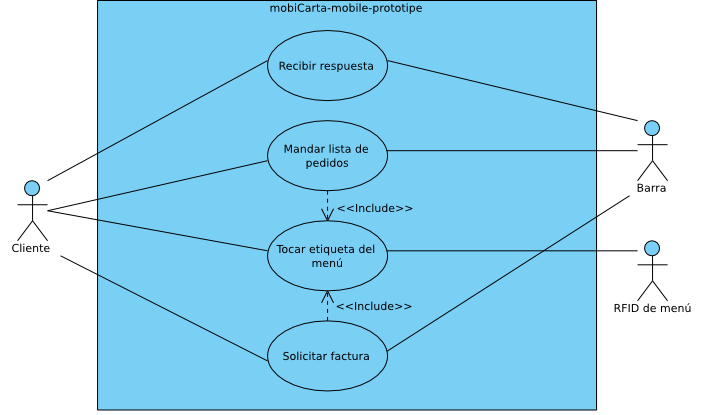
\includegraphics[width=0.9\textwidth]{ucdM-phase5.png}
      \caption{Casos de uso añadidos al prototipo de la aplicación
      móvil en esta iteración.}
      \label{fig:ucdM-phase5}
    \end{center}
  \end{figure}

En este caso se incorporan dos importantes casos de uso:
\begin{itemize}
\item \textbf{Mandar lista de pedidos}. Para solicitar un pedido, antes hay
que elaborar una lista con los productos que el cliente desea. El prototipo
inicial de la aplicación móvil ya permitía realizar la lista de productos
pero no permitía enviarla. La figura \ref{fig:sdM1-phase5} (página
\pageref{fig:sdM1-phase5}) muestra el \textbf{diagrama de secuencia} de este
caso de uso.

  \begin{figure}[!h]
    \begin{center}
      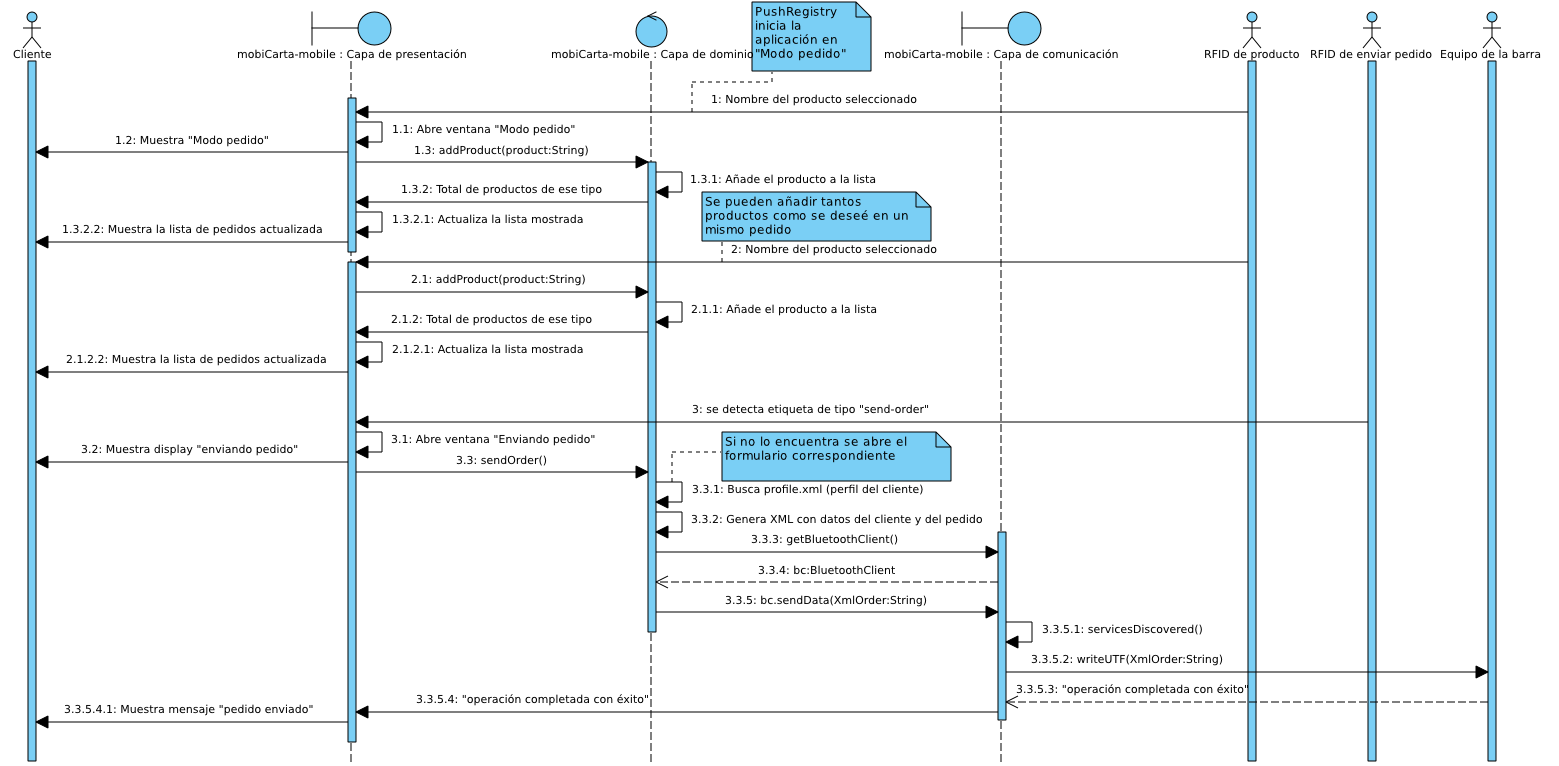
\includegraphics[width=1\textwidth]{sdM1-phase5.png}
      \caption{Diagrama de secuencia del caso de uso \emph{mandar lista
      de pedidos}. En este caso el cliente solicita dos productos.}
      \label{fig:sdM1-phase5}
    \end{center}
  \end{figure}

Cuando el dispositivo móvil contacta con una etiqueta de tipo \emph{product},
la aplicación móvil arranca automáticamente en \emph{modo pedido}. Todas las
etiquetas de tipo \emph{product} contienen el nombre del producto al que
representan. Este nombre aparecerá como el primer elemento de la lista de
productos para el pedido. Cuando el móvil contacta con una segunda etiqueta
\emph{product}, la aplicación comprueba la lista de productos existente; si
el producto ya aparece en la lista, incrementa el número de productos de ese
tipo; si no, el producto se añade a la lista en una nueva línea.

Para enviar el pedido, el usuario debe acercar su móvil a una etiqueta de
tipo \emph{send-order}. En ese momento, la aplicación buscará el archivo
\emph{profile.xml} para extraer la información del usuario y compondrá un
\acs{XML} con estos datos y con la lista de productos elaborada. Por último,
la aplicación buscará el servicio \emph{Bluetooth} ofrecido por la aplicación
de la \emph{barra} y le mandará una cadena con el \acs{XML}. La aplicación
de la \emph{barra} contestará si ha recibido la cadena correctamente.

\item \textbf{Solicitar factura}. El usuario dispone de la opción de conocer,
a través de la aplicación móvil, cuál es el importe que debe abonar por los
pedidos realizados. La figura \ref{fig:sdM2-phase5} (página
\pageref{fig:sdM2-phase5}) muestra el \textbf{diagrama de secuencia} de los
pasos que debe seguir.

  \begin{figure}[!h]
    \begin{center}
      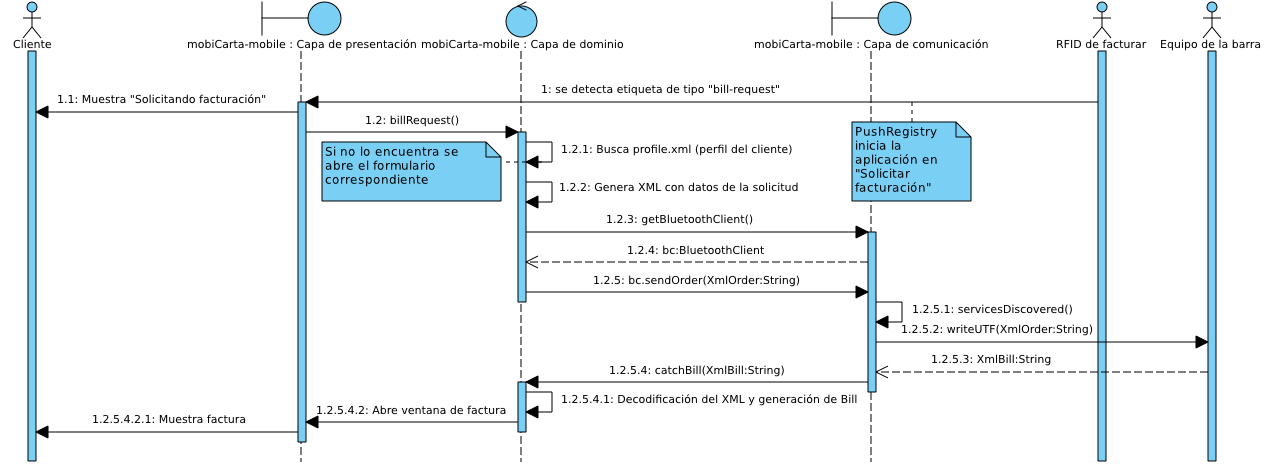
\includegraphics[width=1\textwidth]{sdM2-phase5.png}
      \caption{Diagrama de secuencia del caso de uso \emph{solicitar factura}.}
      \label{fig:sdM2-phase5}
    \end{center}
  \end{figure}

Cuando el dispositivo móvil detecta la presencia de una etiqueta de tipo
\emph{bill-request}, arranca automáticamente la aplicación en \emph{modo
solicitar facturación}. A continuación, la aplicación busca el archivo
\emph{profile.xml} para extraer la información del usuario y con ello componer
un \acs{XML} con el motivo \emph{solicitar facturación}. Este \acs{XML} se
manda al servicio correspondiente de la aplicación de la \emph{barra}. Y,
finalmente, esta responde con un resumen (en \acs{XML}) de la factura de la 
mesa que ocupa el cliente. Este resumen contiene información como: cliente, 
mesa, número de factura, pedidos realizados, subtotal, descuentos, IVA e
importe total.
\end{itemize}

% Meter modificaciones del diagrama de clases del prototipo de la barra
% y del prototipo móvil.

\subsection{Sistema recomendador}
El objetivo del sistema recomendador es ofrecer al cliente una serie de
servicios extra que le incentiven a seguir utilizando la tecnología \acs{NFC}
dentro de dicho establecimiento. Implementar el sistema recomendador implicará
realizar cambios en el prototipo de los servicios web y la base de datos, en
el prototipo del \emph{recibidor} y en el prototipo de la aplicación móvil.
Al término de esta iteración se habrá obtenido la primera versión del prototipo
final del sistema.

\subsubsection{Análisis de requisitos}
Los requisitos que debe satisfacer el sistema recomendador son los siguientes:
\begin{enumerate}
\item El sistema recomendador debe ofrecer la siguiente información al cliente:
  \begin{itemize}
  \item Cuáles son los platos que más ha consumido.
  \item Qué productos de la carta tienen algún descuento.
  \item Teniendo en cuenta los productos favoritos del cliente, qué productos
  similares a estos pueden gustarle.
  \end{itemize}
\item El sistema recomendador será ejecutado por la aplicación de los
servicios web.
\item La base de datos contará con una nueva tabla (\emph{historial}) con el
histórico de pedidos que ha realizado el cliente a lo largo de sus visitas
al restaurante. Esta tabla se utilizará para calcular las recomendaciones para
un cliente.
\item El cliente recibirá las recomendaciones cuando registre su entrada en el
restaurante (vía \emph{Bluetooth}), aunque también podrá consultarlas mientras
está elaborando una lista para un pedido.
\end{enumerate}

\subsubsection{Diseño e implementación}
El diseño del sistema recomendador va a afectar a los servicios web y su
base de datos, a la aplicación del \emph{recibidor} y a la aplicación
móvil.

La aplicación del \emph{recibidor} añade un único caso de uso (figura
\ref{fig:ucdR-phase6}):

  \begin{figure}[!h]
    \begin{center}
      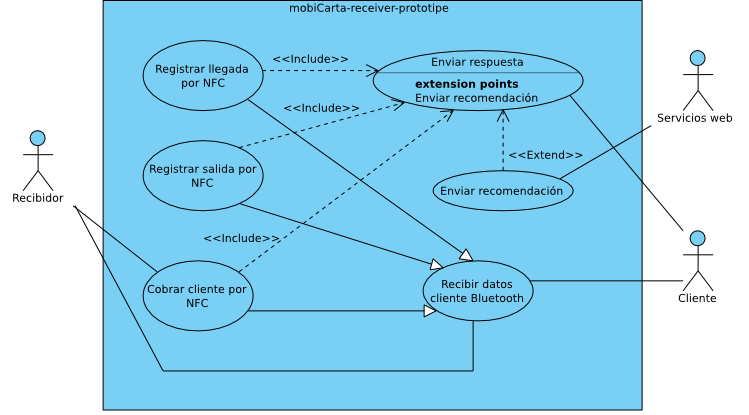
\includegraphics[width=1\textwidth]{ucdR-phase6.png}
      \caption{Casos de uso \emph{enviar recomendación} añadido a la aplicación 
      del \emph{recibidor}.}
      \label{fig:ucdR-phase6}
    \end{center}
  \end{figure}

La aplicación móvil añade dos casos de uso (figura \ref{fig:ucdM-phase6}):

  \begin{figure}[!h]
    \begin{center}
      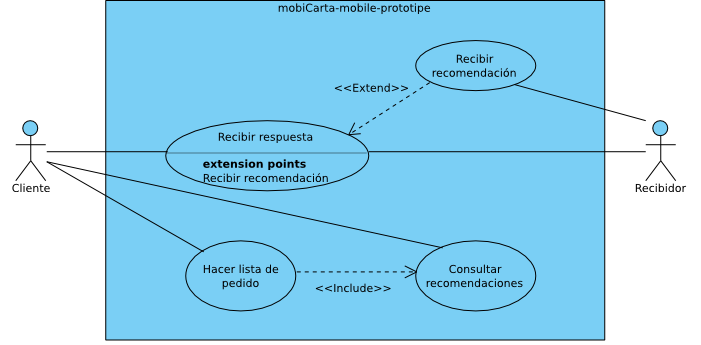
\includegraphics[width=1\textwidth]{ucdM-phase6.png}
      \caption{Se añaden los casos de uso \emph{recibir recomendación} y
      \emph{consultar recomendaciones}.}
      \label{fig:ucdM-phase6}
    \end{center}
  \end{figure}

% Añadir diagrama de secuencia del recomendador en el servicio web, el la
% aplicación de la barra y el la aplicación móvil.

% Insertar esquema de cómo se calculan las recomendaciones.

% Hacer referencia de que en los anexos están los diagramas de clases completos
% de todas las aplicaciones que forman parte del sistema.

\section{Pruebas}
  \subsection{Pruebas unitarias}
% Ya veremos si me da tiempo
  \subsection{Pruebas de campo}
% Decir cómo las he hecho y las conclusiones obtenidas.
% Hacer referencia de que en los anexos están los formularios utilizados para
% tomar nota de lo que piensan los usuarios de las aplicaciones.

\section{Manual de usuario}
% Lo típico: pantallazos y explicaciones...
  \subsection{Servicios web y base de datos}
  \subsection{Aplicación del recibidor}
  \subsection{Aplicación de la barra}
  \subsection{Aplicación móvil}

\section{Diagrama de Gantt del proyecto}
% Por hacer...

\section{Estimación de costes}
% ¿Debo incluir el desarrollo de este prototipo (vamos, de todo el PFC) como
% costes? ¿A qué precio se pagaría el trabajo de un estudiante de ISI entonces?
% Supongo que debo suponer que existen costes para transformar este prototipo
% en una aplicación comercial y que existen unos costes de instalación y 
% mantenimiento; además están los costes de las etiquetas, los terminales,
% las pantallas táctiles, etc.


% Local Variables:
%   coding: utf-8
%   fill-column: 90
%   mode: flyspell
%   ispell-local-dictionary: "american"
%   mode: latex
%   TeX-master: "main"
% End:
